% cvpr_presentation.tex

\documentclass[10pt,red,xcolor=pdftex,dvipsnames,table]{beamer}

\usetheme{DarkConsole}
\usefonttheme{professionalfonts}

\usepackage{bm}
\usepackage{todonotes}
\usepackage{subcaption}
\usepackage{tikz}
\usepackage{tikz-3dplot}
\usepackage{tikzscale}
\usetikzlibrary{arrows,shapes,chains,matrix,positioning}
\usetikzlibrary{scopes,decorations,shadows,backgrounds,fit}
\usetikzlibrary{decorations.pathreplacing,calc,3d,quotes}
\usepackage{pgfmath}
\usepackage{threeparttable}
\usepackage{tcolorbox}
\usepackage{pgfplots}
\usepackage[utf8]{inputenc}

\usepackage{media9}
\newcommand{\includemovie}[3]{%
\includemedia[width=#1,height=#2,activate=pagevisible,deactivate=pageclose,passcontext,addresource=#3,flashvars={source=#3
&autoPlay=true
&loop=true
&controlBarAutoHideTimeout=1
&autoRewind=true
&delay=1
}
]{}{VPlayer.swf}}
 
\setbeamertemplate{title page}
{
	\vbox{}
	\vfill
	\begin{centering}
		{\usebeamerfont{title}\usebeamercolor[fg]{title}\inserttitle}
		\vskip0.2em
		{\usebeamerfont{subtitle}\usebeamercolor[fg]{subtitle}\insertsubtitle}
		\vskip2em\par
		\small\insertauthor\par
		\vskip1em\par
		\small\insertinstitute\par
		\vskip1em\par
		\small CVPR 2019 \vskip1em\par
	\end{centering}
 	\vfill
}

%%%%%% TITLE, AUTHOR, DATE DEFINITIONS %%%%%%

\title[CVPR 2019]{The World's Most Awesome Slides}
\author[Vishnu Boddeti]{Vishnu Boddeti}
\institute[]{Michigan State University}
\date{\today}

\begin{document}
 
\frame{\titlepage}

\begin{frame}{Problem Setting: Adversarial Representation Learning}
\begin{figure}
\centering
\tikzstyle{format} = [draw, thin, fill=blue!40]
\tikzstyle{medium} = [ellipse, draw, thin, fill=green!40, minimum height=2.0em]
\tikzstyle{decision} = [diamond, draw, fill=blue!40, text width=4.5em, text badly centered, node distance=2cm, inner sep=0pt]
\tikzstyle{block} = [rectangle, draw, fill=white!40, text width=3em, rounded corners, minimum height=3em]
\tikzstyle{blockl} = [rectangle, draw=black, fill=blue!40, text width=6em, text centered, rounded corners, minimum height=6em]
\tikzstyle{blocks} = [rectangle, draw=black, fill=blue!40, text width=4em, text centered, rounded corners, minimum height=2em]
\tikzstyle{line} = [draw, -latex']
\tikzstyle{cloud} = [draw,ellipse,fill=red!40,node distance=2cm,minimum height=1.5em]
\tikzstyle{circ} = [draw=black,circle,fill=white!40,node distance=2cm]
\tikzstyle{mybar} = [minimum width=0.02cm, minimum height=0.2cm, rectangle, draw=black]
\begin{tikzpicture}[very thick]
    \uncover<1->{
    \node[blockl, fill=blue!40] (a) {\missingfigure{}};
    \node[blockl, right of=a, node distance=3.2cm, fill=yellow!40] (d) {};
    \node[mybar, right of=d, node distance=2.0cm, fill=green!40] (e) {};
    \node[mybar, above of=e, node distance=0.2cm, fill=green!40] (e1) {};
    \node[mybar, above of=e, node distance=0.4cm, fill=green!40] (e2) {};
    \node[mybar, above of=e, node distance=0.6cm, fill=green!40] (e3) {};
    \node[mybar, below of=e, node distance=0.2cm, fill=green!40] (e3) {};
    \node[mybar, below of=e, node distance=0.4cm, fill=green!40] (e4) {};
    \node[mybar, below of=e, node distance=0.6cm, fill=green!40] (e6) {};
    \node[node distance=1.4cm, above of=d] (d12) {\footnotesize $E(\mathbf{x}, \bm{\theta}_E)$};
    \node[node distance=1.2cm, above of=e3] (d13) {\footnotesize $\mathbf{z}\in \mathbb{R}^d$};}

    \node[right of=d, node distance=2.2cm] (y1) {};
    \node[above of=y1, node distance=0.2cm] (y2) {};
    \node[below of=y1, node distance=0.2cm] (y3) {};
    
    \node[right of=d, node distance=3.3cm] (x1) {};
    \node[above of=x1, node distance=0.8cm] (x2) {};
    \node[below of=x1, node distance=0.8cm] (x3) {};

    \node[right of=d, node distance=4cm] (f1) {};
    \uncover<1->{\node[blocks, above of=f1, node distance=0.8cm, fill=cyan!40] (g1) {\footnotesize {\color{black}$T(\bm{x},\bm{\theta}_T)$}};
    \node[right of=g1, node distance=2.0cm] (g2) {\footnotesize $q_T(t|\bm{z})$};
    \draw[->] (g1) -- (g2);}
    \uncover<1->{\node[blocks, below of=f1, node distance=0.8cm, fill=red!40] (h1) {\footnotesize {\color{black}$A(\bm{x},\bm{\theta}_A)$}};
    \node[right of=h1, node distance=2.0cm] (h2) {\footnotesize $q_A(s|\bm{z})$};
    \draw[->] (h1) -- (h2);}
    
    \uncover<1->{
    \node[circ, right of=a, node distance=3.2cm] (d1) {};
    \node[circ, above of=d1, node distance=0.5cm] (d2) {};
    \node[circ, below of=d1, node distance=0.5cm] (d3) {};
    \node[right of=d1, node distance=0.7cm] (d4) {};
    \node[circ, above of=d4, node distance=0.2cm] (d41) {};
    \node[circ, below of=d4, node distance=0.2cm] (d42) {};
    \node[left of=d1, node distance=0.7cm] (d5) {};
    \node[circ, above of=d5, node distance=0.2cm] (d6) {};
    \node[circ, above of=d5, node distance=0.6cm] (d7) {};
    \node[circ, below of=d5, node distance=0.2cm] (d8) {};
    \node[circ, below of=d5, node distance=0.60cm] (d9) {};
    \draw[help lines, thick] (d1) -- (d41);
    \draw[help lines, thick] (d2) -- (d41);
    \draw[help lines, thick] (d3) -- (d41);
    \draw[help lines, thick] (d1) -- (d42);
    \draw[help lines, thick] (d2) -- (d42);
    \draw[help lines, thick] (d3) -- (d42);
    \draw[help lines, thick] (d6) -- (d1);
    \draw[help lines, thick] (d6) -- (d2);
    \draw[help lines, thick] (d6) -- (d3);
    \draw[help lines, thick] (d7) -- (d1);
    \draw[help lines, thick] (d7) -- (d2);
    \draw[help lines, thick] (d7) -- (d3);
    \draw[help lines, thick] (d8) -- (d1);
    \draw[help lines, thick] (d8) -- (d2);
    \draw[help lines, thick] (d8) -- (d3);
    \draw[help lines, thick] (d9) -- (d1);
    \draw[help lines, thick] (d9) -- (d2);
    \draw[help lines, thick] (d9) -- (d3);

    \draw[->] (a) -- (d);
    \draw[->] (d) -- (e);}

    \uncover<1->{\draw[->, double, thin] (y2) -- (x2);}
    \uncover<1->{\draw[->, double, thin] (y3) -- (x3);}
\end{tikzpicture}
\end{figure}

\vspace{1cm}
\begin{itemize}
	\setlength\itemsep{0.5cm}
	\item<1-> Three player game between:
	\begin{itemize}
		\item<1-> {\color{yellow!40} Encoder} extracts features $\bm{z}$
		\item<1-> {\color{cyan!40} Target Predictor} for desired task from features $\bm{z}$
		\item<1-> {\color{red!40} Adversary} extracts sensitive information from features $\bm{z}$
	\end{itemize}
\end{itemize}
\end{frame}
  
\begin{frame}{Maximum Entropy Adversarial Representation Learning}
	\vspace{0.5cm}
	\begin{tcolorbox}[title=Key Idea]
		Optimize the encoder to maximize entropy of adversary as opposed to minimizing its likelihood.
	\end{tcolorbox}
	\begin{columns}
		\uncover<2->{
		\begin{column}{0.3\textwidth}
			\begin{itemize}
				\item Adversary
			\end{itemize}
			\begin{figure}
			\centering
			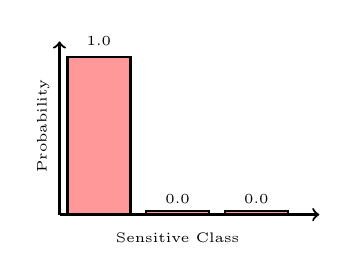
\begin{tikzpicture}[very thick]
				\draw[thick,->] (0,0) -- (0,2.2) node[anchor=south west, yshift=-1.8cm, rotate=90]{\tiny Probability};
				\draw[thick,->] (0,0) -- (3.3,0.0) node[below, xshift=-1.8cm, yshift=-0.1cm]{\tiny Sensitive Class};
				\draw[thick, fill=red!40] (0.1,0) -- (0.9, 0.0) -- (0.9, 2.0) -- (0.1, 2.0) -- cycle;
				\draw[thick, fill=red!40] (1.1,0) -- (1.9, 0.0) -- (1.9, 0.05) -- (1.1, 0.05) -- cycle;
				\draw[thick, fill=red!40] (2.1,0) -- (2.9, 0.0) -- (2.9, 0.05) -- (2.1, 0.05) -- cycle;
				\node at (0.5, 2.2) {\tiny 1.0};
				\node at (1.5, 0.2) {\tiny 0.0};
				\node at (2.5, 0.2) {\tiny 0.0};
			\end{tikzpicture}
			\end{figure}
		\end{column}}

		\uncover<2->{
		\begin{column}{0.3\textwidth}
			\begin{itemize}
				\item Encoder
			\end{itemize}
			\begin{figure}
			\centering
			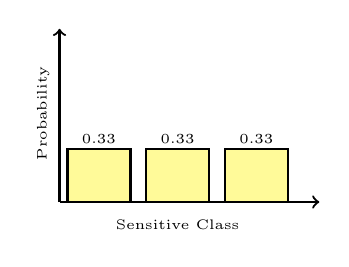
\begin{tikzpicture}[very thick]
				\draw[thick,->] (0,0) -- (0,2.2) node[anchor=south west, yshift=-1.8cm, rotate=90]{\tiny Probability};
				\draw[thick,->] (0,0) -- (3.3,0.0) node[below, xshift=-1.8cm, yshift=-0.1cm]{\tiny Sensitive Class};
				\draw[thick, fill=yellow!40] (0.1,0) -- (0.9, 0.0) -- (0.9, 0.67) -- (0.1, 0.67) -- cycle;
				\draw[thick, fill=yellow!40] (1.1,0) -- (1.9, 0.0) -- (1.9, 0.67) -- (1.1, 0.67) -- cycle;
				\draw[thick, fill=yellow!40] (2.1,0) -- (2.9, 0.0) -- (2.9, 0.67) -- (2.1, 0.67) -- cycle;
				\node at (0.5, 0.8) {\tiny 0.33};
				\node at (1.5, 0.8) {\tiny 0.33};
				\node at (2.5, 0.8) {\tiny 0.33};
			\end{tikzpicture}
			\end{figure}
		\end{column}}

		\uncover<2->{
		\begin{column}{0.3\textwidth}
			\begin{itemize}
				\item Equilibrium
			\end{itemize}
			\begin{figure}
			\centering
			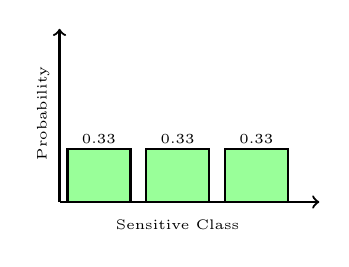
\begin{tikzpicture}[very thick]
				\draw[thick,->] (0,0) -- (0,2.2) node[anchor=south west, yshift=-1.8cm, rotate=90]{\tiny Probability};
				\draw[thick,->] (0,0) -- (3.3,0.0) node[below, xshift=-1.8cm, yshift=-0.1cm]{\tiny Sensitive Class};
				\draw[thick, fill=green!40] (0.1,0) -- (0.9, 0.0) -- (0.9, 0.67) -- (0.1, 0.67) -- cycle;
				\draw[thick, fill=green!40] (1.1,0) -- (1.9, 0.0) -- (1.9, 0.67) -- (1.1, 0.67) -- cycle;
				\draw[thick, fill=green!40] (2.1,0) -- (2.9, 0.0) -- (2.9, 0.67) -- (2.1, 0.67) -- cycle;
				\node at (0.5, 0.8) {\tiny 0.33};
				\node at (1.5, 0.8) {\tiny 0.33};
				\node at (2.5, 0.8) {\tiny 0.33};
			\end{tikzpicture}
			\end{figure}
		\end{column}}
	\end{columns}

	\vspace{0.5cm}
	\uncover<3->{
	Contributions:
	\begin{itemize}
		\item Theoretical analysis of equillibrium and convergence dynamics.
		\item Visualization and empirical evaluation on multiple datasets.
	\end{itemize}}
\end{frame}

\frame{
\frametitle{Summary}
	\begin{itemize}
		\setlength\itemsep{0.5cm}
		\item A striving step towards explicitly controlling information in learned representations.
		\item MaxEnt-ARL: optimize the encoder to maximize entropy of adversary instead of minimizing likelihood.
		\item MaxEnt-ARL is practically effective and enjoys theoretical benefits.
	\end{itemize}

	\uncover<2->{
	\vspace{1cm}
	\begin{tcolorbox}[title=Code:]
    	\url{https://github.com/human-analysis/MaxEnt-ARL.git}
	\end{tcolorbox}
	\vspace{1cm}
	\begin{center}
	    {\color{red!40} \Large More Details: Poster \# 175}
	\end{center}}
}

\end{document}